\documentclass{article}
\usepackage[utf8]{inputenc}
\usepackage[T2A]{fontenc}
\usepackage[utf8]{inputenc}
\usepackage{float}
%\usepackage[russian]{babel}
\usepackage[a4paper, left=10mm, right=10mm, top=20mm, bottom=20mm]{geometry}
\usepackage{natbib}
\usepackage{graphicx}
\usepackage{tabularx}
\usepackage{hyperref}

\title{PSD@CBM FEE and readout (draft, for internal use)}
\author{Finogeev Dmitry, INR RAS}





\begin{document}

\maketitle

Actual version of the document is available at github:
\newline
\url{https://github.com/dfinogee/PSD-readout-manual/raw/main/PSD_readout_manual.pdf}



\tableofcontents


% ###########################################
% ################# PSD FEE #################
% ###########################################
\newpage
\part{PSD FEE boards}


% ###########################################
\section{ADC board}

% ###########################################
\subsection{ADC clock scheme}\label{sec:adc-clock}

% ###########################################
\section{ADC addon}



% ###########################################
\section{ADC data processing}
PSD\_data\_readout component receive data from all ADCs, process waveform and output data in GBT packets. Schematic of component is presented on fig.~\ref{fig:1}.

\begin{figure}[H]
	\centering 
	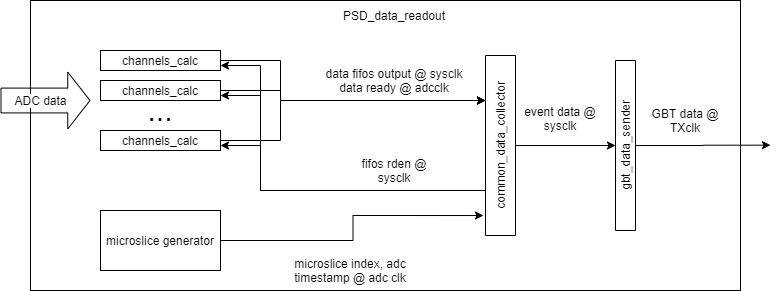
\includegraphics[width=0.8\textwidth]{ADC_readout.png}
	\caption{\label{fig:1} ADC data readout scheme}
\end{figure}



% ###########################################
\subsection{Component channels\_calc}
Channel\_calc component scheme is presented on figure~\ref{fig:2}. ADC data inverted for negative signals, zero level and RMS are calculated and available from slow control.

\begin{figure}[H]
	\centering 
	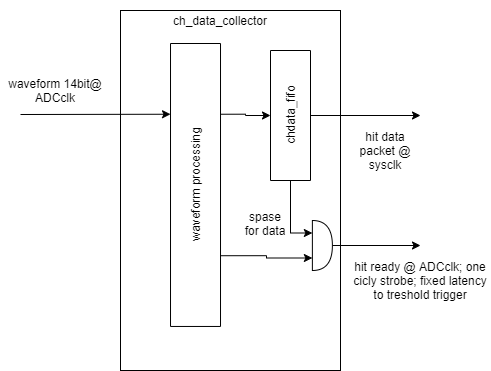
\includegraphics[width=1.0\textwidth]{ADC_event_collection.png}
	\caption{\label{fig:2} Channel data processing scheme}
\end{figure}

Strobe\_generator component forms waveform gate, start and stop signals by threshold crossing taking waveform length and offset parameters. Waveform data that are available from the start (zero level) are latched while strobe. Signal diagram of the component is presented on figure~\ref{fig:3} To reduce the probability of being triggered by a noise event, three neighboring points are compared with threshold. Central point is compared with the threshold value and two side points with half of threshold value.

Waveform offset parameter determine waveform position in gate, if it is 0, first point in waveform strobe is  the point above threshold (the third point compared to half of threshold value). Maximum offset value is 13. Latched baseline level is value before point above threshold.

If one channel in common trigger mask parameter cross threshold, common trigger is generated. All channels in common trigger output parameter take waveform similar to they has threshold crossing together.

\begin{figure}[H]
	\centering 
	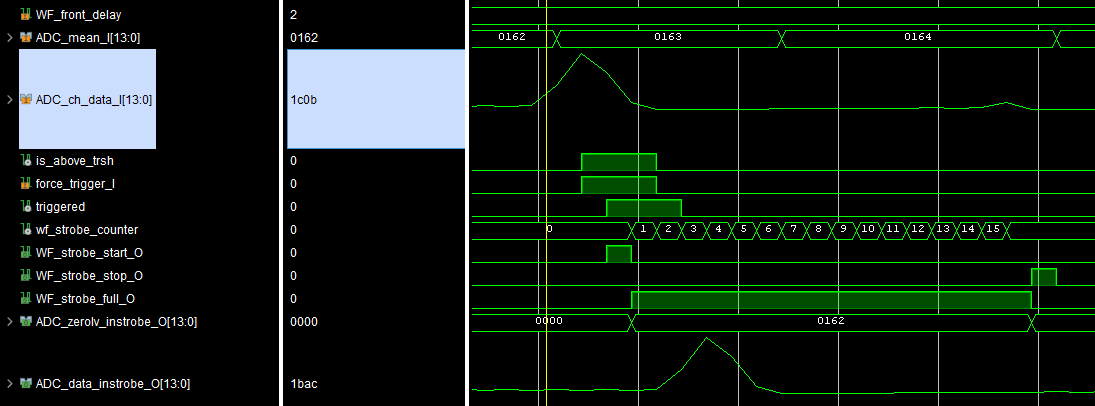
\includegraphics[width=0.8\textwidth]{wf_strobe_diag_sim.png}
	\caption{\label{fig:3} Signal waveform strobe (length 16, offset 3)}
\end{figure}


Ch\_data\_collector store waveform point in raw\_fifo by strobe signal and start waveform data (zero level) by start signal. When charge ready signal raised, charge and start data from header\_fifo stored in data\_fifo as hit packed header. This allow to upgrade charge calculation with fitting procedure and change calculation delay. In next cycle waveform points are read from raw\_fifo and (if sending wf points parameter is set on) stored as hit data in ch\_data\_fifo. After hit packet stored, ready signal raised or dropped signal in case fifo was full and hit packet was dropped. Ready and dropped signals are synchronous to threshold crossing and used for event ADC timestamp.  Signals diagram of the component is presented on figure~\ref{fig:4}. The write size of ch\_data\_fifo should be equal to ceil(calculation\_delay / waveform\_lenght)*waveform\_lenght. The size of ch\_header\_fifo should be ceil(calculation\_delay / waveform\_lenght). Write rate for mentioned fifo is equal to read rate.
In case data-fifo is full while charge ready signal, hit is dropped and dropped-hits counter increased by 1. Dropped-hits counter is available in channel status and reset after each register reading.

Readout-rate component allow to measure hit rate per channel. Waveform-start signals counted with 16bit counter and 70Hz rate. Each 70 Hz cycle, count is stored in 128 shift register. Rate-mean register store the summ of values stored in shift register. Two modes: low-rate and normal are available for rate reading. In normal mode for 16 bit status register available rate-mean[22 downto 7] and result is rate/70Hz. In low-rate mode (channel-low-rate-count bit) rate-mean[15 downto 0] available for status register and result is rate/70*128Hz.

\begin{figure}[H]
	\centering 
	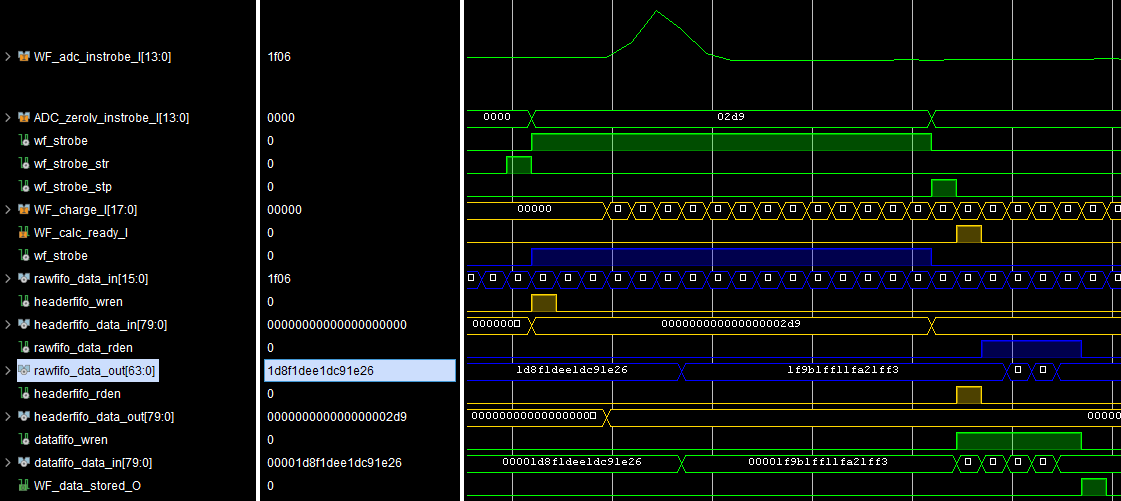
\includegraphics[width=1.0\textwidth]{ADC_ch_data_collector_wave.png}
	\caption{\label{fig:4} Channel data collecting signals}
\end{figure}

Signals could be processed one after another without dead time. If next adc point after waveform gate is higher than threshold, new signal gate is formed. Signal time is next adc cycle after first gate, not is real time of second waveform threshold crossing. Signal diagram for such case is presented on figure~\ref{fig:5}.


\begin{figure}[H]
	\centering 
	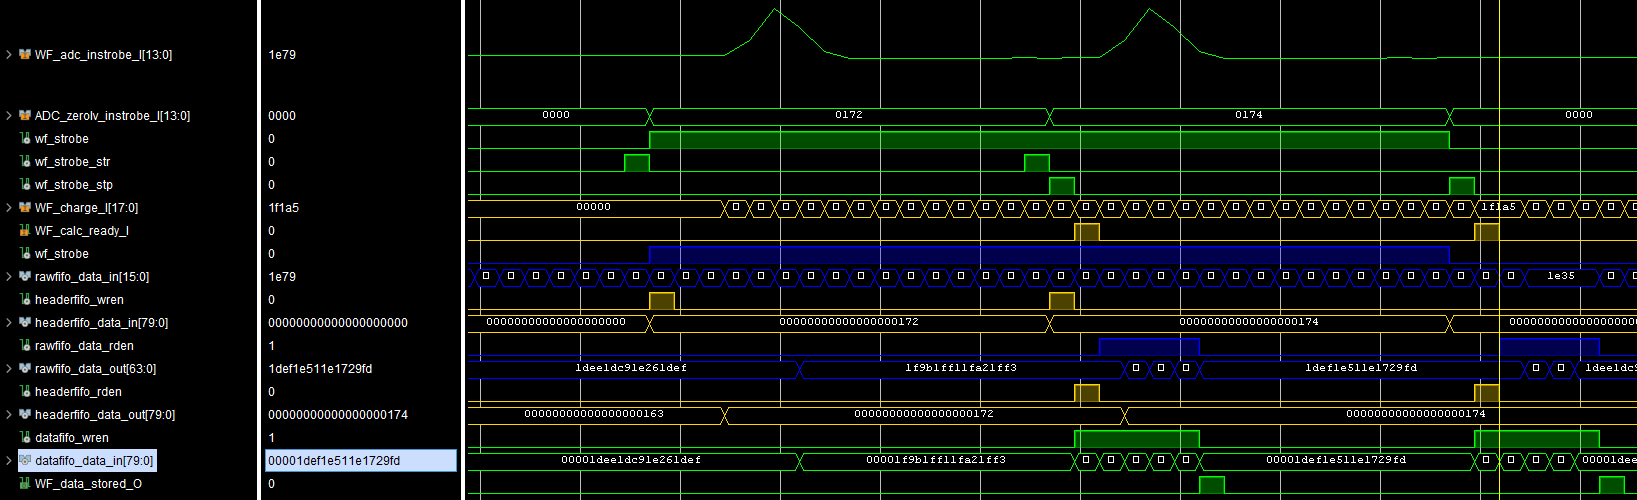
\includegraphics[width=1.0\textwidth]{ADC_ch_data_collector_wave_pileup.png}
	\caption{\label{fig:5} Channel data collecting signals}
\end{figure}



% ###########################################
\subsection{Component common\_data\_collector}
Each channel generate single strobe with fixed latency to threshold crossing indicating waveform measurement. 32 bit strobe word is stored to data\_wf\_calc\_fifo with mc index and ADC timestamp. FSM read stored strobes and collect data from fired channels storing outputs to common\_data\_fifo, each event header word with timing and data size info stored in common\_header\_fifo. Schematic represented on figure ~\ref{fig:3}.

\begin{figure}[H]
	\centering 
	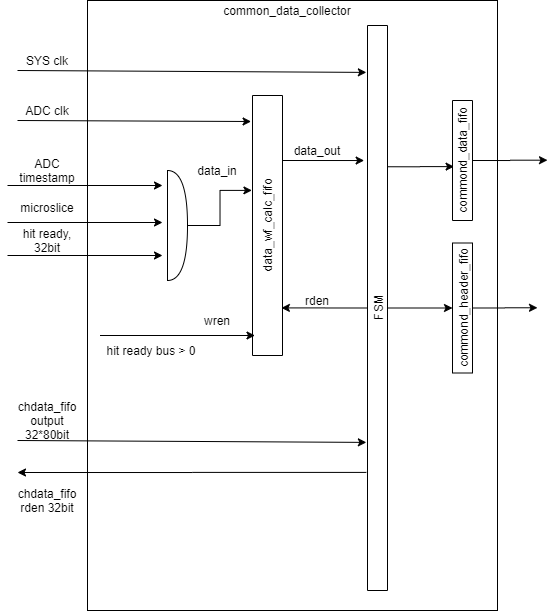
\includegraphics[width=0.5\textwidth]{ADC_common_event_collection.png}
	\caption{\label{fig:6} Data collecting scheme from all channels fifos}
\end{figure}

FSM is switched from wait to start state when data\_wf\_calc\_fifo\_isempty became '0' and fifo output is latched. Priority encoder show next fired channel from strobe and data collected from fired channel to common\_data\_fifo with hit\_packet\_iterator. Input to priory encoder is shifted to bit after fired channel when iterator reach last fired channel. Priority encoder could be equal or less than 32 bit. Simulation outputs presented on figure ~\ref{fig:4}.

\begin{figure}[H]
	\centering 
	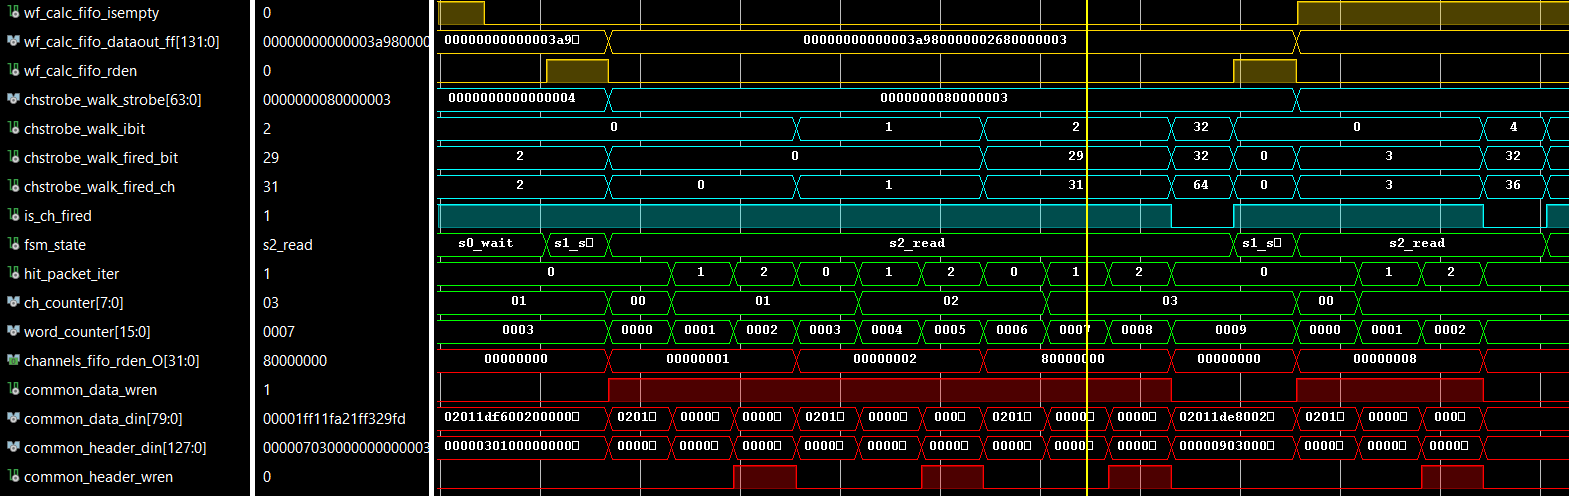
\includegraphics[width=1.0\textwidth]{ADC_common_data_collector_wave.png}
	\caption{\label{fig:7} Data collecting signal from all channels fifos}
\end{figure}

Collecting data from all channels takes two additional FSM cycle. Mean hit rate per channel in case all channels fired is SYSCKL / total channels + 2 cycle / packet length. Test beam: 80MHz / 12 / 5 = 1.3MHz. Final setup: 120 (240) / 32 / 1 = 3.5 (7) MHz.



% ###########################################
\subsection{Component GBT\_data\_sender}

Data stored in common\_data\_fifo in component common\_data\_collector are read by system clock with writing rate. Event and microslice headers are formed by data from common\_header\_fifo. Built GBT data packets are stored in gbt\_data\_fifo and read by GBT TX clock. Signal diagram is presented on figure~\ref{fig:8}. 


\begin{figure}[H]
	\centering 
	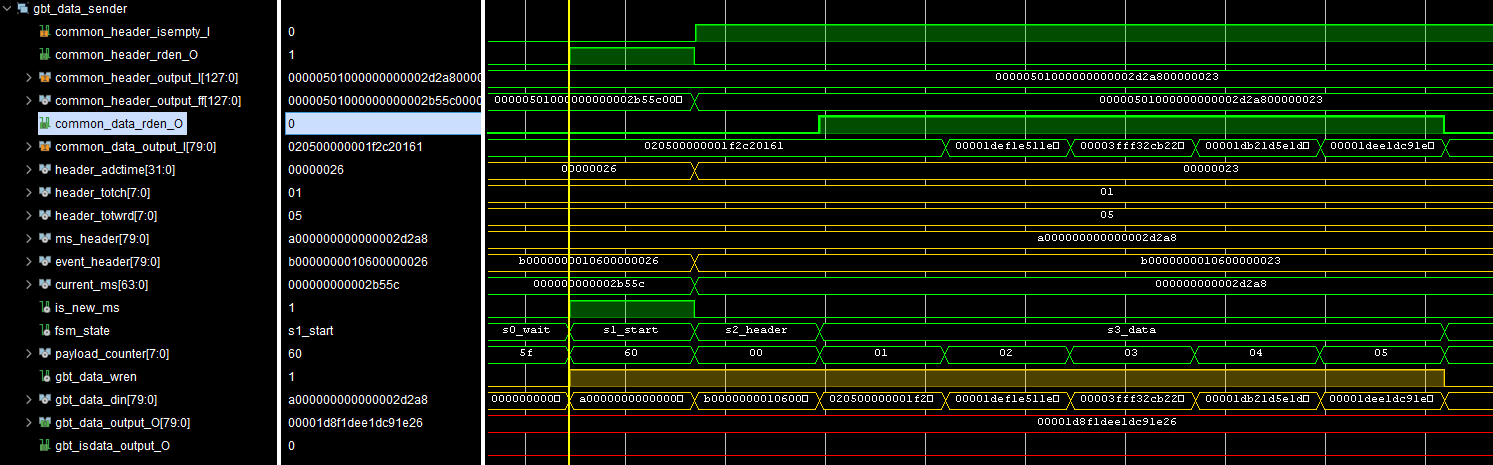
\includegraphics[width=1.0\textwidth]{GBT_sender_wave.png}
	\caption{\label{fig:8} Channel data collecting signals}
\end{figure}

Data rate limit is 80bit X 40MHz = 0.4 GB/s(GBT). Hit rate limit per channel (without microslice word) is 40MHz / 33 (packet length) = 1,2 MHz in case all channels are fired. The rate could be increased to  2.4 MHz hits per channel in case all 32 channels are fired. If one hit data will be less than 40bit event packet will contain 17 GBT words.

GBT packet format is presented on tables: ~\ref{tab1}, ~\ref{tab2}, ~\ref{tab3}

\begin{table}[H]
\centering
\begin{tabular}{| l | l | l | l | l | l | l | l | l |}
\hline
word type & 79 .. 76 & 75 .. 72 & 71 .. 64 & 63 .. 48 & 47 .. 40 & 39 .. 32 & 31 .. 16 & 15 .. 0 \\ \hline
ms header & 0xA & \multicolumn{2}{c|}{0x0}  & \multicolumn{5}{c|}{ms index} \\ \hline
event header & 0xB & ADC idx** & \multicolumn{2}{c|}{0x0} & n fired channels & words in packet * & \multicolumn{2}{c|}{adc time} \\ \hline
hit header & \multicolumn{8}{c|}{hit header (tab.~\ref{tab1})} \\ \hline
hit data & \multicolumn{8}{c|}{hit data (tab.~\ref{tab2})} \\ \hline
hit data & \multicolumn{8}{c|}{hit data (tab.~\ref{tab2})} \\ \hline
hit data & \multicolumn{8}{c|}{hit data (tab.~\ref{tab2})} \\ \hline
hit data & \multicolumn{8}{c|}{hit data (tab.~\ref{tab2})} \\ \hline
  & \multicolumn{8}{c|}{ ... } \\ \hline

event header & 0xB & ADC idx** & \multicolumn{2}{c|}{0x0} & n fired channels & words in packet * & \multicolumn{2}{c|}{adc time} \\ \hline
  & \multicolumn{7}{c|}{ ... } \\ \hline

\end{tabular}
\caption{GBT data format. [* number of GBT words in event packet: event header + all hit packets] [** ADC board index] \label{tab1}}
\end{table}

\begin{table}[H]
\centering
\begin{tabular}{| l | l | l | l | l | l |}
\hline
word & 79 .. 72 & 71 .. 64 & 63 .. 36 & 35 .. 16 & 15 .. 0 \\ \hline
1 & channel &words in packet *& 0x0 & signal charge & waveform zero level \\ \hline
\end{tabular}
\caption{hit packet header. [* total GBT words in hit packet: header + data words]\label{tab2}}
\end{table}

\begin{table}[H]
\centering
\begin{tabular}{| l | l | l | l | l | l |}
\hline
word & 79 .. 64 & 63 .. 48 & 47 .. 32 & 31 .. 16 & 15 .. 0 \\ \hline
1 & 0x0 & waveform point n & waveform point n+1 & waveform point n+2 & waveform point n+3 \\ \hline
\end{tabular}
\caption{hit packet data word.\label{tab3}}
\end{table}

Reserved first 8 bits in GBT data flow:
\begin{itemize}
\item 0x0:0x20 - hit header ch number

\item 0x3 - hit data word (DOTO)

\item 0xA - microslice header

\item 0xB - event header

\item 0xC - CRI FLIM iface mcs delimiter word

\item 0xE - status packet word

\item 0xF - control packet word
\end{itemize}



% ###########################################
\section{ADC control}



% ###########################################
\subsection{ADC control units}\label{sec:adc-control}
Status and Control of ADC are 64 arrays each of 32 bit words.
ADC control system include 4 firmware units: gbt-control-sender, gbt-control-reader, gbt-status-sender, gbt-status-reader. ADC control and monitoring strategy is describe in sec.~\ref{cri-adc-ctrl-desc}

gbt-control-sender is placed on CRI side and send control packet (129 X 16bit) via gbt to ADC. Packet could be send at any time and is not in conflict with microslice flow to ADC. gbt-control-reader receive control packet, and update registers array with raising "updated" strobe.

\begin{table}[H]
\centering
\begin{tabular}{| l | l |}
\hline
word & value \\ \hline
0 & 0xABBA \\ \hline
1 & control(0)(15 .. 0) \\ \hline
2 & control(0)(31 .. 16) \\ \hline
3 & control(1)(15 .. 0) \\ \hline
4 & control(1)(31 .. 16) \\ \hline
\multicolumn{2}{|c|}{....} \\ \hline
127 & control(63)(15 .. 0) \\ \hline
128 & control(63)(31 .. 16) \\ \hline
\end{tabular}
\caption{Control packet to ADC.\label{tab4}}
\end{table}

gbt-status-sender send status or control registers from ADC (packet 32 X 80bit).  Status/control packet is prioritized to data flow, and gbt-data-fifo is not read while transaction. Status and control words starts with 0xE and 0xF accordingly to be distinguished from data flow. 

Sending of control or status packets could be initiated by CRI side with 0xABBB and 0xABBC codes in MSB of RX data.

\begin{table}[H]
\centering
\begin{tabular}{| l | l | l | l | l |}
\hline
 bits & 79 .. 76 & 75 .. 64 & 63 .. 32 & 31 .. 0 \\ \hline
word & code & addr & reg1 & reg0 \\ \hline
0 & E & 0 & status(1) & status(0) \\ \hline
1 & E & 2 & status(3) & status(2) \\ \hline
\multicolumn{5}{|c|}{....} \\ \hline
31 & E & 30 & status(31) & status(30) \\ \hline
\end{tabular}
\caption{Status packet from ADC.\label{tab4}}
\end{table}

\begin{table}[H]
\centering
\begin{tabular}{| l | l | l | l | l |}
\hline
 bits & 79 .. 76 & 75 .. 64 & 63 .. 32 & 31 .. 0 \\ \hline
word & code & addr & reg1 & reg0 \\ \hline
0 & F & 0 & control(1) & control(0) \\ \hline
1 & F & 2 & control(3) & control(2) \\ \hline
\multicolumn{5}{|c|}{....} \\ \hline
31 & F & 30 & control(31) & control(30) \\ \hline
\end{tabular}
\caption{Control packet from ADC.\label{tab4}}
\end{table}

gbt-status-reader read each gbt word stars with 0xE or 0xF and update control or status registers. Two counters indicate the time passed from last update. Read back control register is compared with actual on CRI side. 



% ###########################################
\subsection{Addon I2C control}



% ###########################################
\subsection{ADC Control registers}

\begin{table}[H]
\centering
\begin{tabular}{| l | l | l | l | l | l | l | l | l | l | l |}
\hline
addr & 31 .. 30 & 29 .. 28 & 27 .. 24 & 23 .. 20 & 19 .. 16 & 15 .. 14 & 13 .. 12 & 11 .. 8 & 7 .. 4 & 3 .. 0 \\ \hline
0 & 0x0 & \multicolumn{4}{c|}{threshold ch1} & 0x0 & \multicolumn{4}{c|}{threshold ch0} \\ \hline
1 & 0x0 & \multicolumn{4}{c|}{threshold ch3} & 0x0 & \multicolumn{4}{c|}{threshold ch2} \\ \hline
2 & 0x0 & \multicolumn{4}{c|}{threshold ch5} & 0x0 & \multicolumn{4}{c|}{threshold ch4} \\ \hline
3 & 0x0 & \multicolumn{4}{c|}{threshold ch7} & 0x0 & \multicolumn{4}{c|}{threshold ch6} \\ \hline
4 & 0x0 & \multicolumn{4}{c|}{threshold ch9} & 0x0 & \multicolumn{4}{c|}{threshold ch8} \\ \hline
5 & 0x0 & \multicolumn{4}{c|}{threshold ch11} & 0x0 & \multicolumn{4}{c|}{threshold ch10} \\ \hline
6 & 0x0 & \multicolumn{4}{c|}{threshold ch13} & 0x0 & \multicolumn{4}{c|}{threshold ch12} \\ \hline
7 & 0x0 & \multicolumn{4}{c|}{threshold ch15} & 0x0 & \multicolumn{4}{c|}{threshold ch14} \\ \hline
8 & 0x0 & \multicolumn{4}{c|}{threshold ch17} & 0x0 & \multicolumn{4}{c|}{threshold ch16} \\ \hline
9 & 0x0 & \multicolumn{4}{c|}{threshold ch19} & 0x0 & \multicolumn{4}{c|}{threshold ch18} \\ \hline
10 & 0x0 & \multicolumn{4}{c|}{threshold ch21} & 0x0 & \multicolumn{4}{c|}{threshold ch20} \\ \hline
11 & 0x0 & \multicolumn{4}{c|}{threshold ch23} & 0x0 & \multicolumn{4}{c|}{threshold ch22} \\ \hline
12 & 0x0 & \multicolumn{4}{c|}{threshold ch25} & 0x0 & \multicolumn{4}{c|}{threshold ch24} \\ \hline
13 & 0x0 & \multicolumn{4}{c|}{threshold ch27} & 0x0 & \multicolumn{4}{c|}{threshold ch26} \\ \hline
14 & 0x0 & \multicolumn{4}{c|}{threshold ch29} & 0x0 & \multicolumn{4}{c|}{threshold ch28} \\ \hline
15 & 0x0 & \multicolumn{4}{c|}{threshold ch31} & 0x0 & \multicolumn{4}{c|}{threshold ch30} \\ \hline
\end{tabular}
\caption{ADC channels threshold control.\label{tab4}}
\end{table}

\begin{table}[H]
\centering
\begin{tabular}{| l | l | l | l | l | l | l | l | l |}
\hline
addr & 31 .. 28 & 27 .. 24 & 23 .. 20 & 19 .. 16 & 15 .. 12 & 11 .. 8 & 7 .. 4 & 3 .. 0 \\ \hline
16 & \multicolumn{2}{c|}{0x0} & \multicolumn{2}{c|}{status ch sel} & waveform length 0..3 [(reg+1)*4] & strobe offset 0..12 & \multicolumn{2}{c|}{control bits} \\ \hline
17 & \multicolumn{8}{c|}{negative channel mask ibit = ich} \\ \hline
18 & \multicolumn{8}{c|}{I2C HV bus} \\ \hline
19 & \multicolumn{8}{c|}{microslice gen counter@25ns} \\ \hline
20 & \multicolumn{8}{c|}{microslice period} \\ \hline
21 & \multicolumn{8}{c|}{common trigger OR mask} \\ \hline
22 & \multicolumn{8}{c|}{common trigger output} \\ \hline
23 & \multicolumn{8}{c|}{trigger pulser rate [count @ ADC clock] (0x0 = off)} \\ \hline
24 & \multicolumn{4}{c|}{status send rate (0x0 = off)}& \multicolumn{4}{c|}{control send rate (0x0 = off)} \\ \hline
25 & \multicolumn{8}{c|}{common trigger AND mask} \\
\hline
\end{tabular}
\caption{ADC readout control.}
\end{table}

\begin{table}[H]
\centering
\begin{tabular}{| l | l |}
\hline
bit & description \\ \hline
0 & send waveform \\ \hline
1 & ms gen standalone \\ \hline
2 & readout fsm reset \\ \hline
3 & errors reset \\ \hline
4 & channel low rate count \\ \hline
5 & reset channels drop counter \\ \hline
\end{tabular}
\caption{Control bits\label{tab6}}
\end{table}

\begin{table}[H]
\centering
\begin{tabular}{| l | l | l | l | l | l | l |}
\hline
addr & 31 .. 25 & 24 .. 24 & 23 .. 23 & 22 .. 16 & 15 .. 8 & 7 .. 0 \\ \hline
18 & 0x0 & start & WR & i2c dev addr & mem addr & data \\ \hline
\end{tabular}
\caption{HV control via I2C.\label{tab7}}
\end{table}



% ###########################################
\subsection{ADC Status registers}

Status registers map is presented on table \ref{tab8}. 

\begin{table}[H]
\centering
\begin{tabular}{| l | l | l | l | l | l | l | l | l | l | l |}
\hline
addr & 31 .. 30 & 29 .. 28 & 27 .. 24 & 23 .. 20 & 19 .. 16 & 15 .. 14 & 13 .. 12 & 11 .. 8 & 7 .. 4 & 3 .. 0 \\ \hline
0 & \multicolumn{10}{c|}{microslice index 31 .. 0}\\ \hline
1 & \multicolumn{10}{c|}{microslice index 63 .. 32}\\ \hline
2 & \multicolumn{10}{c|}{ADC time}\\ \hline
3 & \multicolumn{5}{c|}{RX wrclk err cnt} & \multicolumn{5}{c|}{RX err frclk cnt} \\ \hline
4 & \multicolumn{5}{c|}{RX err detect cnt} & \multicolumn{5}{c|}{I2C HV bus}\\ \hline
5 & \multicolumn{8}{c|}{0x0} & \multicolumn{2}{c|}{temp} \\ \hline
6 & \multicolumn{5}{c|}{sel. channel baseline rms} & \multicolumn{5}{c|}{sel. channel baseline}\\ \hline
7 & \multicolumn{5}{c|}{sel. channel dropped hits} & \multicolumn{5}{c|}{sel. channel hit rate}\\ \hline
8 & \multicolumn{5}{c|}{GBT event dropped} & \multicolumn{5}{c|}{GBT fifo count}\\ \hline
\end{tabular}
\caption{ADC channels threshold control.\label{tab8}}
\end{table}

\begin{table}[H]
\centering
\begin{tabular}{| l | l | l | l | l | l | l | l | l |}
\hline
addr & 15 .. 10 & 9 .. 9 & 8 .. 8 & 7 .. 0 \\ \hline
4 & 0x0 & error ack & busy & DATA \\ \hline
\end{tabular}
\caption{HV status via I2C.\label{tab9}}
\end{table}

Status registers comments:
\begin{itemize}
\item RX err detect cnt - counter@RXclk of RX error detected bit.

\item RX err frclk cnt - counter@RXclk of state when frame clock is not ready.

\item RX wrclk err cnt - counter@RXclk of state when word clock is not ready.
\end{itemize}




% ###########################################
% ################# PSD CRI #################
% ###########################################
\newpage
\part{CRI-PSD firmware}

\section{ADC - CRI operation}

ADC - CRI communication scheme is presented on fig.~\ref{fig:adc-cri}. 

\begin{figure}[H]
	\centering 
	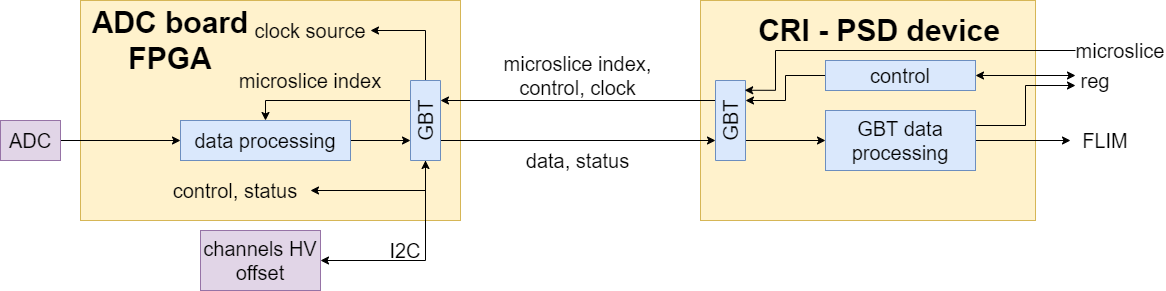
\includegraphics[width=1.0\textwidth]{CRI_PSD_spec.png}
	\caption{\label{fig:adc-cri} ADC - CRI GBT connection}
\end{figure}

GBT-FPGA on ADC board side recover RX clock (see ~\ref{sec:adc-clock}), microslice (64 bit@40MHz each GBT word) and control packets (see ~\ref{sec:adc-control}). Microslice index transported to ADC clock domain (synchronous to RX clock) and each ADC cycle in microslice numerated with adc time index. Measured hits labeled with microslice + adc time indexes and sent to CRI via GBT TX. Control and monitor of data taking, MPPC HV adjustment and MPPC board temperature control is available via GBT control packets.

TODO: update with 2 FPGAs



% ###########################################
\subsection{PSD CRI operation}



% ###########################################
\subsection{CRI - ADC control strategy}\label{sec:cri-adc-ctrl}
Implementation details are described in sec.~\ref{sec:adc-control}

adc-control-sender unit placed in CRI receive mapped adc control registers (64X32bit) from AGWB "psd-adc". By software command all registers could be sent to ADC. After each transaction of control packet ADC send back control register. adc-status-reader unit read control and status packet from ADC on CRI side. Status packets received from ADC updates status on AGWB "psd-adc". Received control packets compared with actual control registers from "psd-adc" and "match" signal indicate correctness of ADC configuration.
ADC reset cycle (FSM or errors) must be done in 4 writes (here and below several fields writes counted as single command):

\begin{itemize}
\item[1] write 0x1 to reset register
\item[2] trigger sending of control packet
\item[3] write 0x0 to reset register
\item[4] trigger sending of control packet
\end{itemize}

Control and status packets could be sent periodically, that allow only read AGWB status registers for ADC monitoring. Also control and status packets could be requested by CRI side, in that case monitoring can be done with one write command (trigger status request) and one read command of status. 

To save registers space, channel status (base level, RMS, hits dropped, hits rate, 64 bits in total) presents in status register map only for one channel. Number of monitored channel is controlled with field "mon-ch-sel". After each time the field is changed on ADC side, status packet sent to CRI automatically. That allow to monitor channel status in 3 command:

\begin{itemize}
\item[1] write numger of monitored channel to register
\item[2] trigger sending of control packet
\item[3] read status fields of channel status
\end{itemize}

Also status packets sent to CRI automatically after each I2C operation that allow to configure addon register in 5 commands:

\begin{itemize}
\item[1] write data for I2C transation (start = 0)
\item[2] trigger sending of control packet
\item[3] write start to 1
\item[4] trigger sending of control packet
\item[5] read I2C status
\end{itemize}

TODO: In future some of operation could be implemented on firmware level:
 
\begin{itemize}
\item Reset cycle could be automated on ADC and CRI sides for single write AGWB command
\item ADC control packet could be sent automatically after changing of registers (with timeout) and ADC configuration mismatch while writing new control values could be processed on CRI side. That will allow just write new configuration on software level.
\item Errors could be reset automatically after sending from ADC and stored and alarmed on CRI side
\item Channel status map could be received automatically with low rate update, representing full channels status table in AGWB
\item I2C operation could be automated with full addon control and status registers map in AGWB

Also, to do not reduce data rate with status registers, packets could be sent via 4 bits of slow-control bus.

\end{itemize}



% ###########################################
\section{PSD CRI data processing}

\begin{figure}[H]
	\centering 
	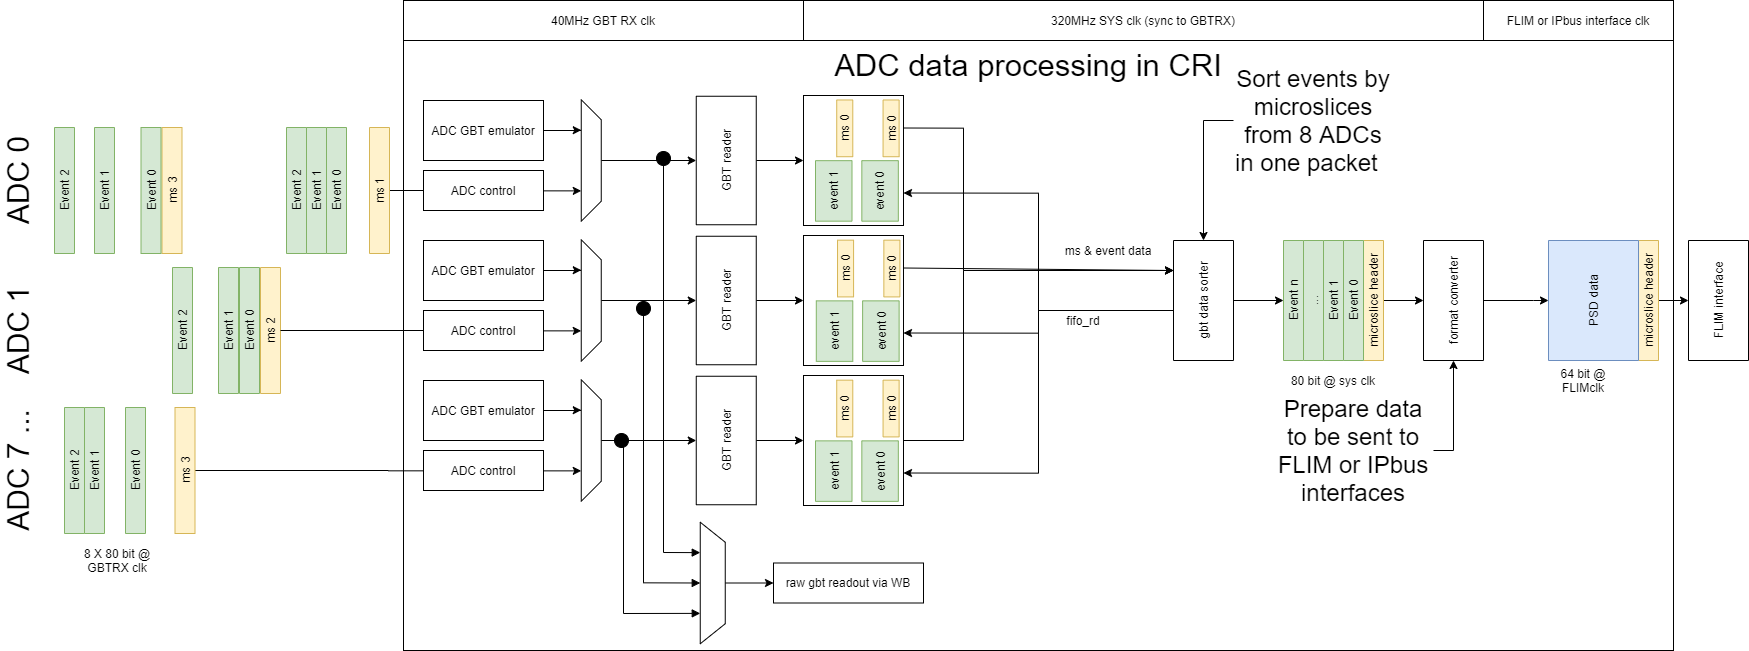
\includegraphics[width=1.0\textwidth]{CRI_data_sort_2.png}
	\caption{\label{fig:cri-data-process} PSD data processing in CRI}
\end{figure}

Figure ~\ref{fig:cri-data-process} present PSD data processing flow. Each ADC board is connected to psd-device with 2 GBT links. There are 4 psd-devices per SLR, 16 GBT links, 8 psd-devices, 2 SLRs in total. Each gbt link is connected to ADC-control, adc-gbt-emu and data-reader units. adc-gbt-emu mute gbt link and emulate adc gbt packets for readout tests purposes (see sec.~\ref{sec:gbt-emu}). adc-control translate adc control and status registers to AGWB (see sec.~\ref{sec:cri-adc-ctrl}). data-reader unit read adc data packets, drop corrupted data and provide each packet with microslice header in separate fifo (see sec.~\ref{sec:data-reader}). Also adc-reader can mute any gbt link. data-sorter unit (see sec.~\ref{sec:data-sorter}) reads data and header buffers from data-reader and sort data by microslice intervals. data-sorter throttle data flow in case FLIM interface is not ready to data transport. While correct operation only data-sorter should throttle data, all other units are able transport data at full 2 gbt links load. Two slow readout units are available for calibration and test: raw-gbt-readout (see sec.~\ref{sec:gbt-rd}) and data-readout (see sec.~\ref{sec:data-rd}). raw-gbt-readout allow to take data as they received from adc board including control packets. It was implemented as one of the first units of PSD-CRI, now it is rudimentary and can be used for debug. data-readout transport sorted and throttled data for tests and calibration purposes.

TODO: data throttling description



% ###########################################
\subsection{ADC GBT emulator}\label{sec:gbt-emu}
adc-gbt-emu generates adc data packets with variable event and hit load in frequency range 1/107Hz ... 20MHz.
Hit header contains microslice index and hit data contains continuous hit counter. adc-gbt-emu is inserted before data-reader and mute gbt link if it is on.

adc-gbt-emu control:
\begin{itemize}
\item turn\_on - mute input gbt link and output generated data if is on.
\item adc\_id - adc board index placed in event header
\item event\_rate is number of GBT clock cycles between packets (from start to start of packet). If previous packet was not sent, and is time to generate new one, new one is skipped.
\item event\_len - number of hits per event 1 ... 255. Emulate fired channels.
\item hit\_len - number of hit words, including hit header 1 ... 255. Emulate waveform data
\end{itemize}

Emulator FSM is based on three counters, simulation signals diagram is presented on figure \ref{fig:gbt-emu-sg}; generated data format is presented on figure \ref{tab:gbt-emu-format}.

\begin{figure}[H]
	\centering 
	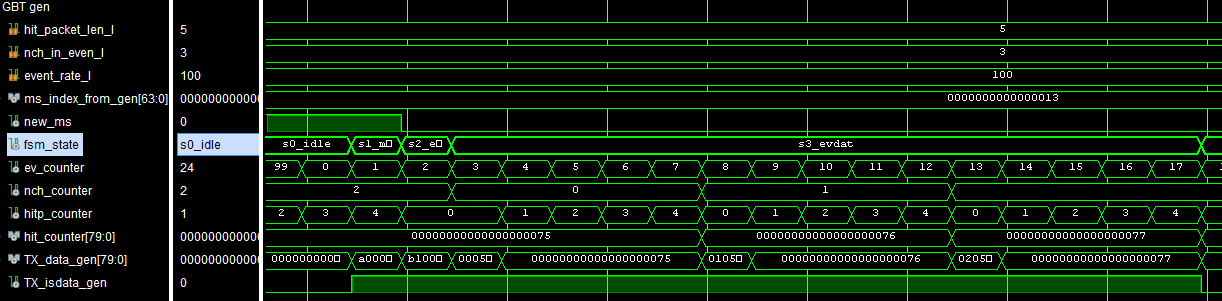
\includegraphics[width=1.0\textwidth]{ADC_GBT_emu_waves.png}
	\caption{\label{fig:gbt-emu-sg} ADC GBT emulator signals}
\end{figure}

\begin{table}[H]
\centering
\begin{tabular}{| l | l | l | l | l | l | l | l | l |}
\hline
word type & 79 .. 76 & 75 .. 72 & 71 .. 64 & 63 .. 48 & 47 .. 40 & 39 .. 32 & 31 .. 16 & 15 .. 0 \\ \hline
ms header & 0xA & \multicolumn{2}{c|}{0x0}  & \multicolumn{5}{c|}{ms index} \\ \hline
event header & 0xB & ADC idx** & \multicolumn{2}{c|}{0x0} & n hits & packet len * & \multicolumn{2}{c|}{0x0} \\ \hline
hit header & \multicolumn{2}{c|}{hit number} & words in hit packet *** & \multicolumn{5}{c|}{ms index} \\ \hline
hit data & \multicolumn{8}{c|}{hit counter [79 ..0]} \\ \hline
hit data & \multicolumn{8}{c|}{hit counter [79 ..0]} \\ \hline
hit data & \multicolumn{8}{c|}{hit counter [79 ..0]} \\ \hline
hit data & \multicolumn{8}{c|}{hit counter [79 ..0]} \\ \hline
  & \multicolumn{8}{c|}{ ... } \\ \hline

event header & 0xB & ADC idx** & \multicolumn{2}{c|}{0x0} & n hits & packet len * & \multicolumn{2}{c|}{0x0} \\ \hline
  & \multicolumn{7}{c|}{ ... } \\ \hline

\end{tabular}
\caption{GBT data format. [* number of GBT words in event packet: event header + all hit packets] [** ADC board index] [*** total words in hit packet, including hit header]\label{tab:gbt-emu-format}}
\end{table}



% ###########################################
\subsection{ADC GBT reader}\label{sec:data-reader}
ADC GBT reader reads GBT packets from one GBT link and store its to fifo event\_fifo. With last packet data word header word pushed to separate fifo header\_ fifo with packet length and microslice index. Event packet skipped when one of fifos is full. After reset fsm starts wait microslice header. Packets reads according to size in header and fsm wait next packet or microslice header. If next word after packet is neither ms or packet header, fsm starts wait ms header. Data drop info state is not implemented yet. Signal diagram is presented on figure \ref{fig:11}. 

\begin{figure}[H]
	\centering 
	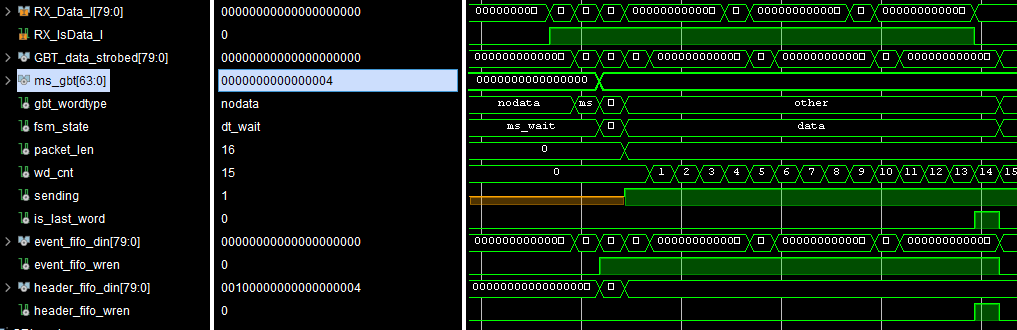
\includegraphics[width=1.0\textwidth]{ADC_GBT_reader_wave.png}
	\caption{\label{fig:11} ADC GBT packets reader}
\end{figure}



% ###########################################
\subsection{GBT Data Sorter component}\label{sec:data-sorter}
Components header\_fifo and event\_fifo from adc-gbt-readers for all gbt links are connected to gbt-data-sorter component. Each new microslice value collected in ms-fifo. FSM switch thought all gbt links and read all one by one links with microslice less or equal to current microslice. Data for links with equal microslice to current-ms output from the sorter, for links with less microslice data is dropped. When all links have ms higher than current ms or are empty means that all data for current microslie are read. Such condition starts counter to wait data from all links. Then counter reach value 127, FSM swithced to next-ms state. Next microslice read from fifo and header with new ms value sent to output stream. Signal diagram presented on figure \ref{fig:10} Output data represent combined GBT packets from all GBT link. All events from GBT links for one microslice follows one after another. Data for different microslices divided by microslice header with format 0xDAF0 + microslice (64bit). 

\begin{figure}[H]
	\centering 
	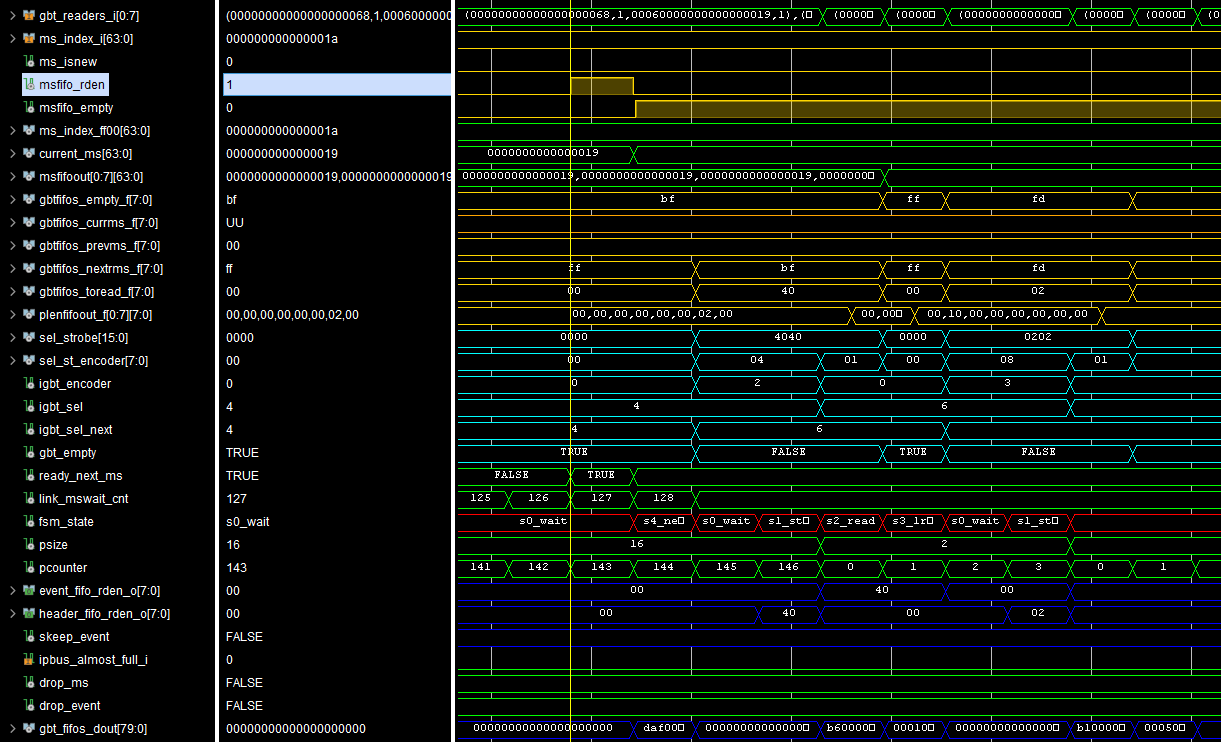
\includegraphics[width=1.0\textwidth]{gbt-sorter-waves.png}
	\caption{\label{fig:10} gbt-data-sorter signals diagram: mew ms read and event sent from one link }
\end{figure}



% ###########################################
\subsection{Calibration readout}\label{sec:data-rd}
IPbus-face-component read data stream from gbt-data-sorter and resize data to width 32 bit. Data stream from gbt-data-sorter stored in fifo-ipbus-face with 80bit write width and 160 read width. Output 160bit word divided in 5 32bit words. Each IPbus read cycle counter 0..4 increased by one, fifo-ipbus-face readed when counter equal 4 and ipbus-read signal is up. While reading empty fifo-ipbus-face all bits are '1'. Signals diagram is presented on figure \ref{fig:11}.

\begin{figure}[H]
	\centering 
	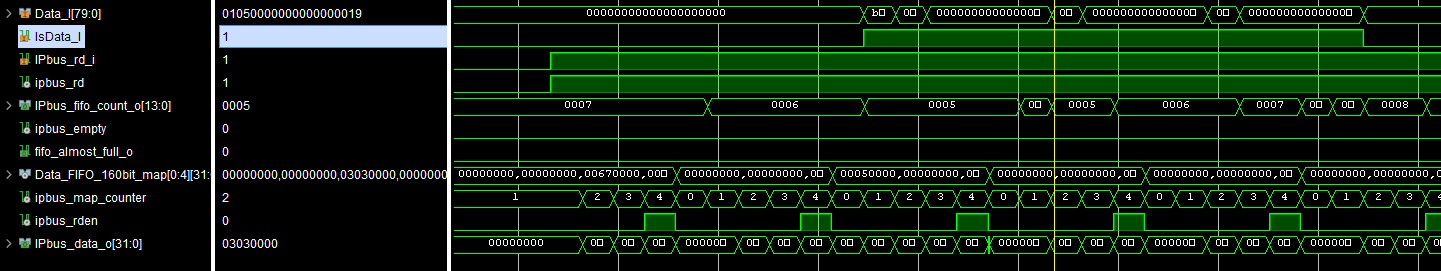
\includegraphics[width=1.0\textwidth]{ipbus-face-waves.png}
	\caption{\label{fig:11} IPbus-face signals diagram }
\end{figure}



% ###########################################
\subsection{Raw GBT readout}\label{sec:gbt-rd}



% ###########################################
\subsection{PSD FLIM interface}\label{sec:flim-iface}



% ###########################################
\subsection{PSD CRI FIFOs usage}



% ###########################################
% ################# PSD EvB #################
% ###########################################
\newpage
\part{PSD evaluation board}

\subsection{EvB control reg}
\begin{table}[H]
\centering
\begin{tabular}{| l | l |}
\hline
range & description \\ \hline
0 .. 63 & EvB control \\ \hline
64 .. 127 & ADC control \\ \hline
128 .. 191 & EvB status \\ \hline
192 .. 255 & ADC status \\ \hline
256 & EvB GBT readout \\ \hline
257 & EvB readout fifo count \\ \hline
\end{tabular}
\caption{EvB registers mapping\label{tab6}}
\end{table}

\begin{table}[H]
\centering
\begin{tabular}{| l | l | l | l | l | l | l | l | l |}
\hline
addr & 31 .. 28 & 27 .. 24 & 23 .. 20 & 19 .. 16 & 15 .. 12 & 11 .. 8 & 7 .. 4 & 3 .. 0 \\ \hline
0 & \multicolumn{6}{c|}{0x0}  & \multicolumn{2}{c|}{control word} \\ \hline
1 & \multicolumn{8}{c|}{microslice gen counter@25ns}  \\ \hline
2 & \multicolumn{8}{c|}{microslice period}  \\ \hline
\end{tabular}
\caption{Evaluation board control registers.\label{tab11}}
\end{table}

\begin{table}[H]
\centering
\begin{tabular}{| l | l |}
\hline
bit & description \\ \hline
0 & data processing reset \\ \hline
1 & error reset \\ \hline
\end{tabular}
\caption{Control word bits\label{tab12}}
\end{table}



\begin{table}[H]
\centering
\begin{tabular}{| l | l | l | l | l | l | l | l | l |}
\hline
addr & 31 .. 28 & 27 .. 24 & 23 .. 20 & 19 .. 16 & 15 .. 12 & 11 .. 8 & 7 .. 4 & 3 .. 0 \\ \hline
0 & \multicolumn{3}{c|}{0x0} & control status  & \multicolumn{4}{c|}{GBT status} \\ \hline
1 & \multicolumn{4}{c|}{sorter ms dropped}  & \multicolumn{4}{c|}{sorter hit dropped} \\ \hline
2 & \multicolumn{4}{c|}{gbt reader link 1 ms dropped}  & \multicolumn{4}{c|}{gbt reader link 0 ms dropped} \\ \hline
3 & \multicolumn{4}{c|}{status age}& \multicolumn{4}{c|}{control age} \\ \hline

\end{tabular}
\caption{Evaluation board status registers.\label{tab13}}
\end{table}

\begin{table}[H]
\centering
\begin{tabular}{| l | l |}
\hline
bit & description \\ \hline
0 & MGT phalin cpll lock \\ \hline
1 & RX word clock ready \\ \hline
2 & RX frame clock ready \\ \hline
3 & MGT link ready \\ \hline
4 & TX reset done \\ \hline
5 & TX FSM reset done \\ \hline
6 & RX ready \\ \hline
7 & RX error detected \\ \hline
8 & RX error latched \\ \hline
\end{tabular}
\caption{GBT status bits\label{tab14}}
\end{table}


\begin{table}[H]
\centering
\begin{tabular}{| l | l | l |}
\hline
bit & addr & description \\ \hline
0 & 16 & control readback correct \\ \hline

\end{tabular}
\caption{control status bits\label{tab14}}
\end{table}







\end{document}

